

\section{Πρόσθεση στο Δυαδικό}
Οι αριθμητικές πράξεις σε αριθμούς εκφρασμένου σε μία συγκεκριμένη βάση ακολουθούν τους ίδιους κανόνες
με αυτούς του δεκαδικού συστήματος, χρησιμοποιώντας σε κάθε περίπτωση μόνο τα διαθέσιμα ψηφία του κάθε
συστήματος. Στα πλαίσια αυτής της διπλωματικής χρησιμοποιείται το δυαδικό σύστημα εφόσον κύριο θέμα 
της είναι η αρχιτεκτονική μελέτη με σκοπό την επιτάχυνση των δυαδικών αθροιστών υπολοίπου.





\subsection{Πρόσθεση δύο ψηφίων}
Στην πρόσθεση δύο διάδικων ψηφίων $x+y$ υπάρχουν τέσσερις πιθανές περιπτώσεις σύμφωνα με το συνδιασμό
των τιμών που παίρνει το κάθε ψηφίο (0 ή 1). Στην περίπτωση $0+0$ το αποτέλεσμα είναι προφανώς μηδέν 
και ίδιο με εκείνο του δεκαδικού συστήματος. Οι περιπτώσεις $0+1$ και $1+0$ έχουν κοινό αποτέλεσμα, 
ίσο με ένα και αυτό οφείλεται στην προσεταιριστική ιδιότητα της πρόσθεσης, η οποία ισχύει σε όλα
τα αριθμητικά συστήματα. Τελευταία περίπτωση είναι και η πιο περίπλοκη, όπου $1+1$ έχει άθροισμα μηδέν
και ένα κρατούμενο. Στον πίνακα \ref{tb:HA_truth_table} παρουσιάζεται ο πίνακας αληθείας, δηλαδή ο 
πίνακας που περιγράφει την συμπεριφορά των εξόδων, στην περίπτωση αυτή το άθροισμα (sum) και το 
κρατούμενο ($c_out$), σύμφωνα με κάθε πιθανό συνδυασμό των εισόδων x και y.


\begin{multicols}{2}
% Table Half Adder
%------------------------------------------
\begin{table}[H]
\centering
 \begin{tabular}{||c c | c c||} 
 \hline
 x & y & sum & $c_{out}$ \\ [0.5ex] 
 \hline\hline
 0 & 0 & 0 & 0 \\ 
 \hline
 0 & 1 & 1 & 0 \\
 \hline
 1 & 0 & 1 & 0 \\
 \hline
 1 & 1 & 0 & 1 \\
 \hline
\end{tabular}
\caption{Half Adder Truth Table}
 \label{tb:HA_truth_table}
\end{table}


% Figure
% HA-Schematic
%--------------------------------------------
\begin{figure}[H]
\centering
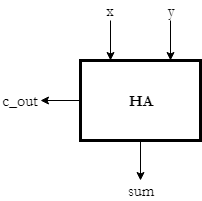
\includegraphics[scale=0.6]{HA.png}
\caption{Half-Adder schematic}
\label{HASchematic}
\end{figure}

\end{multicols}

Το παραπάνω σύστημα ονομάζεται ημιαθροιστής ή Half-Adder (HA) , έχει δυο εισόδους τις x και y και δυο εξόδους τις $c_{out}$ και sum και οι έξοδοι σύμφωνα με τον πίνακα αληθείας περιγράφονται από τις παρακάτω συναρτήσεις άλγεβρας Μπουλ :\\
\begin{equation}
\begin{split}
    sum &= x \oplus y \\ 
    c_{out} &= x * y
\end{split}
\end{equation}\\



Από τον ημιαθροιστής δομείται ο πλήρης αθροιστής ή Full-Adder (FA) με τρεις εισόδους x, y, z , δυο εξόδους sum και $c_{out}$ και λειτουργία αντίστοιχη του FA με την διαφορά πως ο FA προσθέτει τρία δυαδικά ψηφιά \\
\begin{multicols}{2}
\begin{table}[H]
\centering
 \begin{tabular}{||c c c | c c||} 
 \hline
 x & y & z & sum & $c_{out}$ \\ [0.5ex] 
 \hline\hline
 0 & 0 & 0 & 0 & 0 \\ 
 \hline
 0 & 0 & 1 & 1 & 0 \\
 \hline
 0 & 1 & 0 & 1 & 0 \\
 \hline
 0 & 1 & 1 & 0 & 1 \\
 \hline
 1 & 0 & 0 & 1 & 0 \\ 
 \hline
 1 & 0 & 1 & 0 & 1 \\
 \hline
 1 & 1 & 0 & 0 & 1 \\
 \hline
 1 & 1 & 1 & 1 & 1 \\
 \hline
\end{tabular}
\caption{Full Adder Truth Table}
\label{table:2}
\end{table}
% Figure
% FA-Schematic
%--------------------------------------------
\begin{figure}[H]
\centering
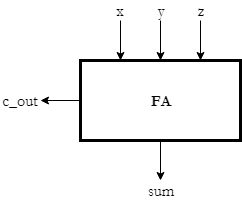
\includegraphics[scale=0.3]{FA.png}
\caption{Full-Adder schematic}
\label{FASchematic}
\end{figure}
\end{multicols}
και οι εξισώσεις των εξόδων είναι :
\begin{equation}
\begin{split}
    sum &= x \oplus y \oplus z \\
    c_{out} &= ( x * y ) + ( x * z ) + ( z * y )
\end{split}
\end{equation}




% 
%------------------------------------------------------------
\subsection{Πρόσθεση δυαδικών αριθμών}

Η πρόσθεση δυο δυαδικών αριθμών A και Β των n δυαδικών ψηφίων το κάθε ένα είναι 
μια επέκταση της πρόσθεσης μεταξύ ψηφίων που παρουσιάστηκε προηγουμένως τροφοδοτώντας 
το κρατούμενο εισόδου των προηγούμενων σημαντικών ψηφίων στην είσοδο του πλήρη αθροιστή 
των επομένων .

% Figure
% FA-Schematic
%--------------------------------------------
\begin{figure}[H]
\centering
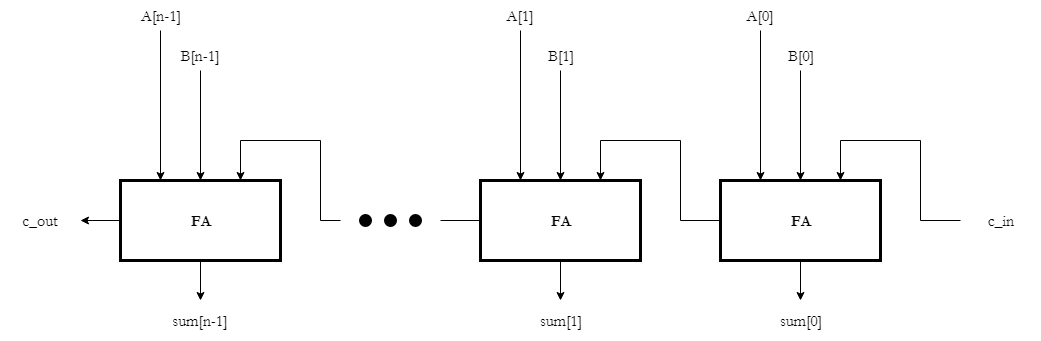
\includegraphics[width=\textwidth]{IntAdder.png}
\caption{Integer-Adder schematic}
\label{IntegerAdderSchematic}
\end{figure}




